\apendice{Documentación de usuario}

\section{Introducción}

En esta sección se enumeran los requisitos que debe cumplir el usuario para poder usar la aplicación, se explica el proceso de instalación y se ofrece un manual de usuario completo para aprender a usarla. 

\section{Requisitos de usuarios}

Para poder instalar y usar la aplicación el dispositivo del usuario debe complir los siguientes requisitos: 

\begin{itemize}
	\item Contar con una versión de Android 6 (\textit{Marshmallow}) o superior, la cual corresponde con la API 23 de Android. 
	\item Permitir la instalación de aplicaciones de orígenes desconocidos~\cite{origenesdesconocidos}. Para ello: 
	\begin{enumerate}
		\item Ir a los ajustes del dispositivo. 
		\item A la opción de \textbf{Seguridad} o \textbf{Privacidad} según la versión. 
		\item Activar la opción \textbf{Orígenes desconocidos}. 
	\end{enumerate}
	\item Contar con conexión a internet. 
\end{itemize}

Además, para poder entrar en la aplicación deberá tener un usuario y una contraseña asignados. 

\section{Instalación}

La instalación de una aplicación Android es muy sencilla. Solo es necesario pasar el archivo \textbf{SmartBeds.apk} al sistema de ficheros del dispositivo Android y seleccionarlo. En caso de tener activada la opción de permitir la instalación de aplicaciones de orígenes desconocidos y contar con el suficiente espacio de almacenamiento la aplicación se instalará automáticamente. 

Se recuerda que el archivo .apk se encuentra en el repositorio del proyecto\footnote{\url{https://github.com/aog0036/TFG-SmartBeds}}, en la ruta \textbf{/android/app/release}.

\section{Manual del usuario}

En esta sección se ofrece un manual para el uso de todas las funcionalidades de la aplicación. 

\subsection{Iniciar sesión}

Al ejecutar la aplicación desde el dispositivo Android la primera pantalla que se muestra es la de Iniciar Sesión. En esta pantalla se nos pide un nombre de usuario y una contraseña para acceder al sistema. Se debe: 

\begin{enumerate}
	\item Introducir el nombre de usuario. 
	\item Introducir la contraseña. 
	\item Pulsar el botón <<Iniciar sesión>>. 
\end{enumerate}

En caso de haber introducido valores correctos se accederá a la siguiente pantalla, en caso contrario un cuadro de diálogo nos indicará que el usuario o la contraseña introducidos no son correctos. 

Si el usuario introducido tiene un rol de administrador la siguiente pantalla será el \textbf{Menú de administración}. Si tiene un rol de usuario la siguiente pantalla será la de \textbf{Visualización de camas}. 

\begin{figure}[H]
	\centering
	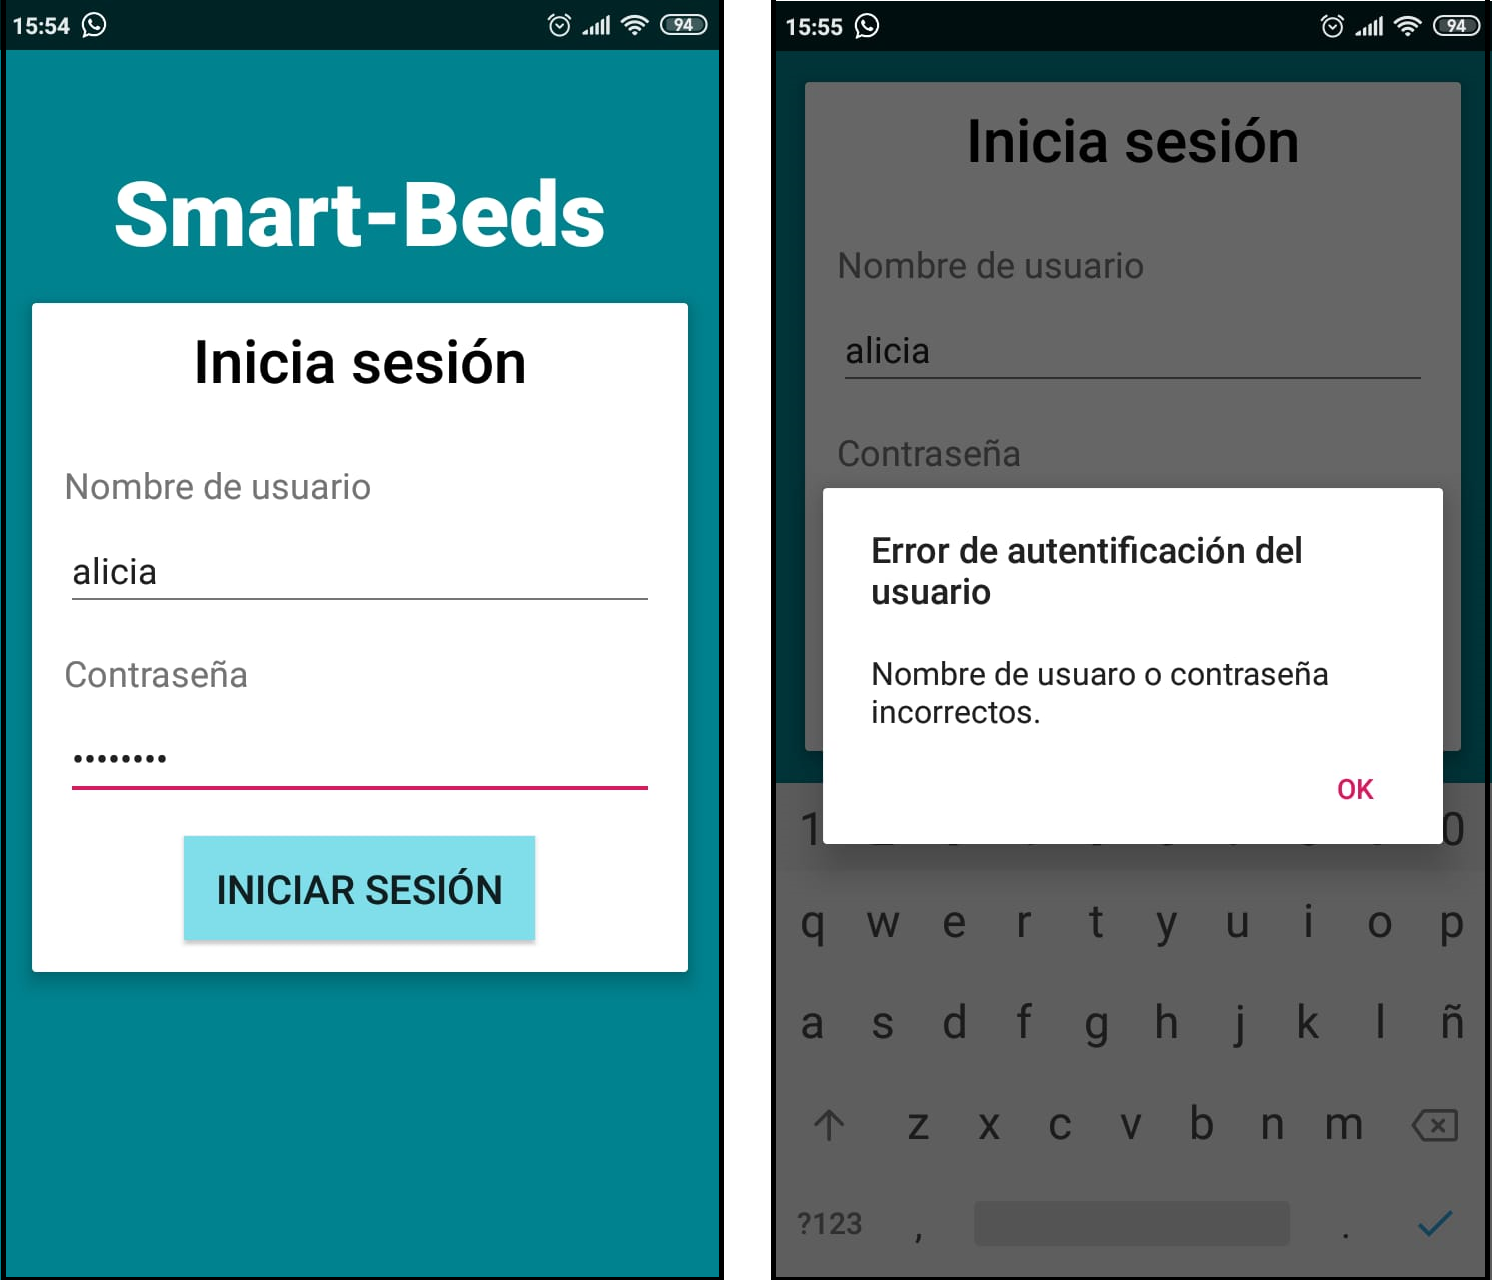
\includegraphics[width=0.7\textwidth]{../img/iniciasesion.png}
	\caption{Iniciar sesión.}
	\label{fig:iniciasesion}
\end{figure}

\subsection{Menú de administración}

Este menú solo está disponible si el usuario tiene un rol de administrador. En él puedes escoger a qué función de la aplicación deseas acceder: \textbf{Gestión de usuarios}, \textbf{Gestión de camas} o \textbf{Visualización de camas}. 

\begin{figure}[H]
	\centering
	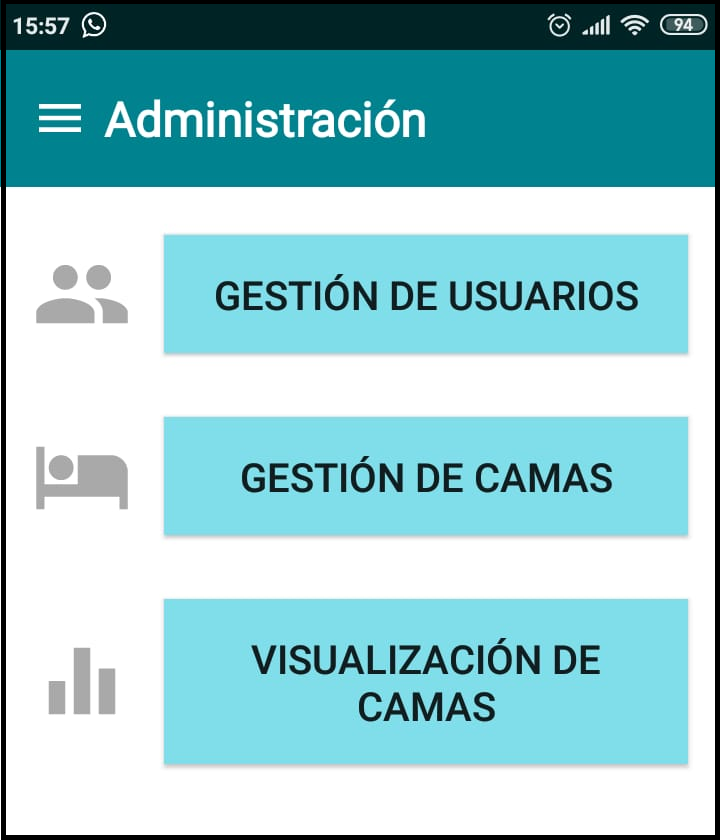
\includegraphics[width=0.4\textwidth]{../img/menudeadministracion.png}
	\caption{Menú de administración.}
	\label{fig:menudeadministracion}
\end{figure}

\subsection{Gesión de usuarios}

Esta pantalla solo está disponible si el usuario tiene un rol de administrador. En esta pantalla se muestra una lista de todos los usuarios registrados en el sistema. Al mantener pulsado uno se muestran las opciones disponibles: \textbf{Cambiar contraseña} y \textbf{Eliminar}.

\begin{itemize}
	\item Si escogemos \textbf{Cambiar contraseña} se muestra una pantalla donde debemos introducir dos veces la nueva contraseña y pulsar el botón <<Cambiar contraseña>>.
	\item Si escogemos \textbf{Eliminar} aparece un cuadro de diálogo preguntando al usuario si desea eliminar de forma permanente al usuario seleccionado. 
	\item Para \textbf{añadir un nuevo usuario} al sistema debemos pulsar en el símbolo <<+>> en la esquina inferior derecha de la pantalla, la cual nos llevará a una pantalla donde deberemos introducir el nombre de usuario y la contraseña del nuevo usuario, y pulsar el botón <<Añadir usuario>>. 
\end{itemize}  

\begin{figure}[H]
	\centering
	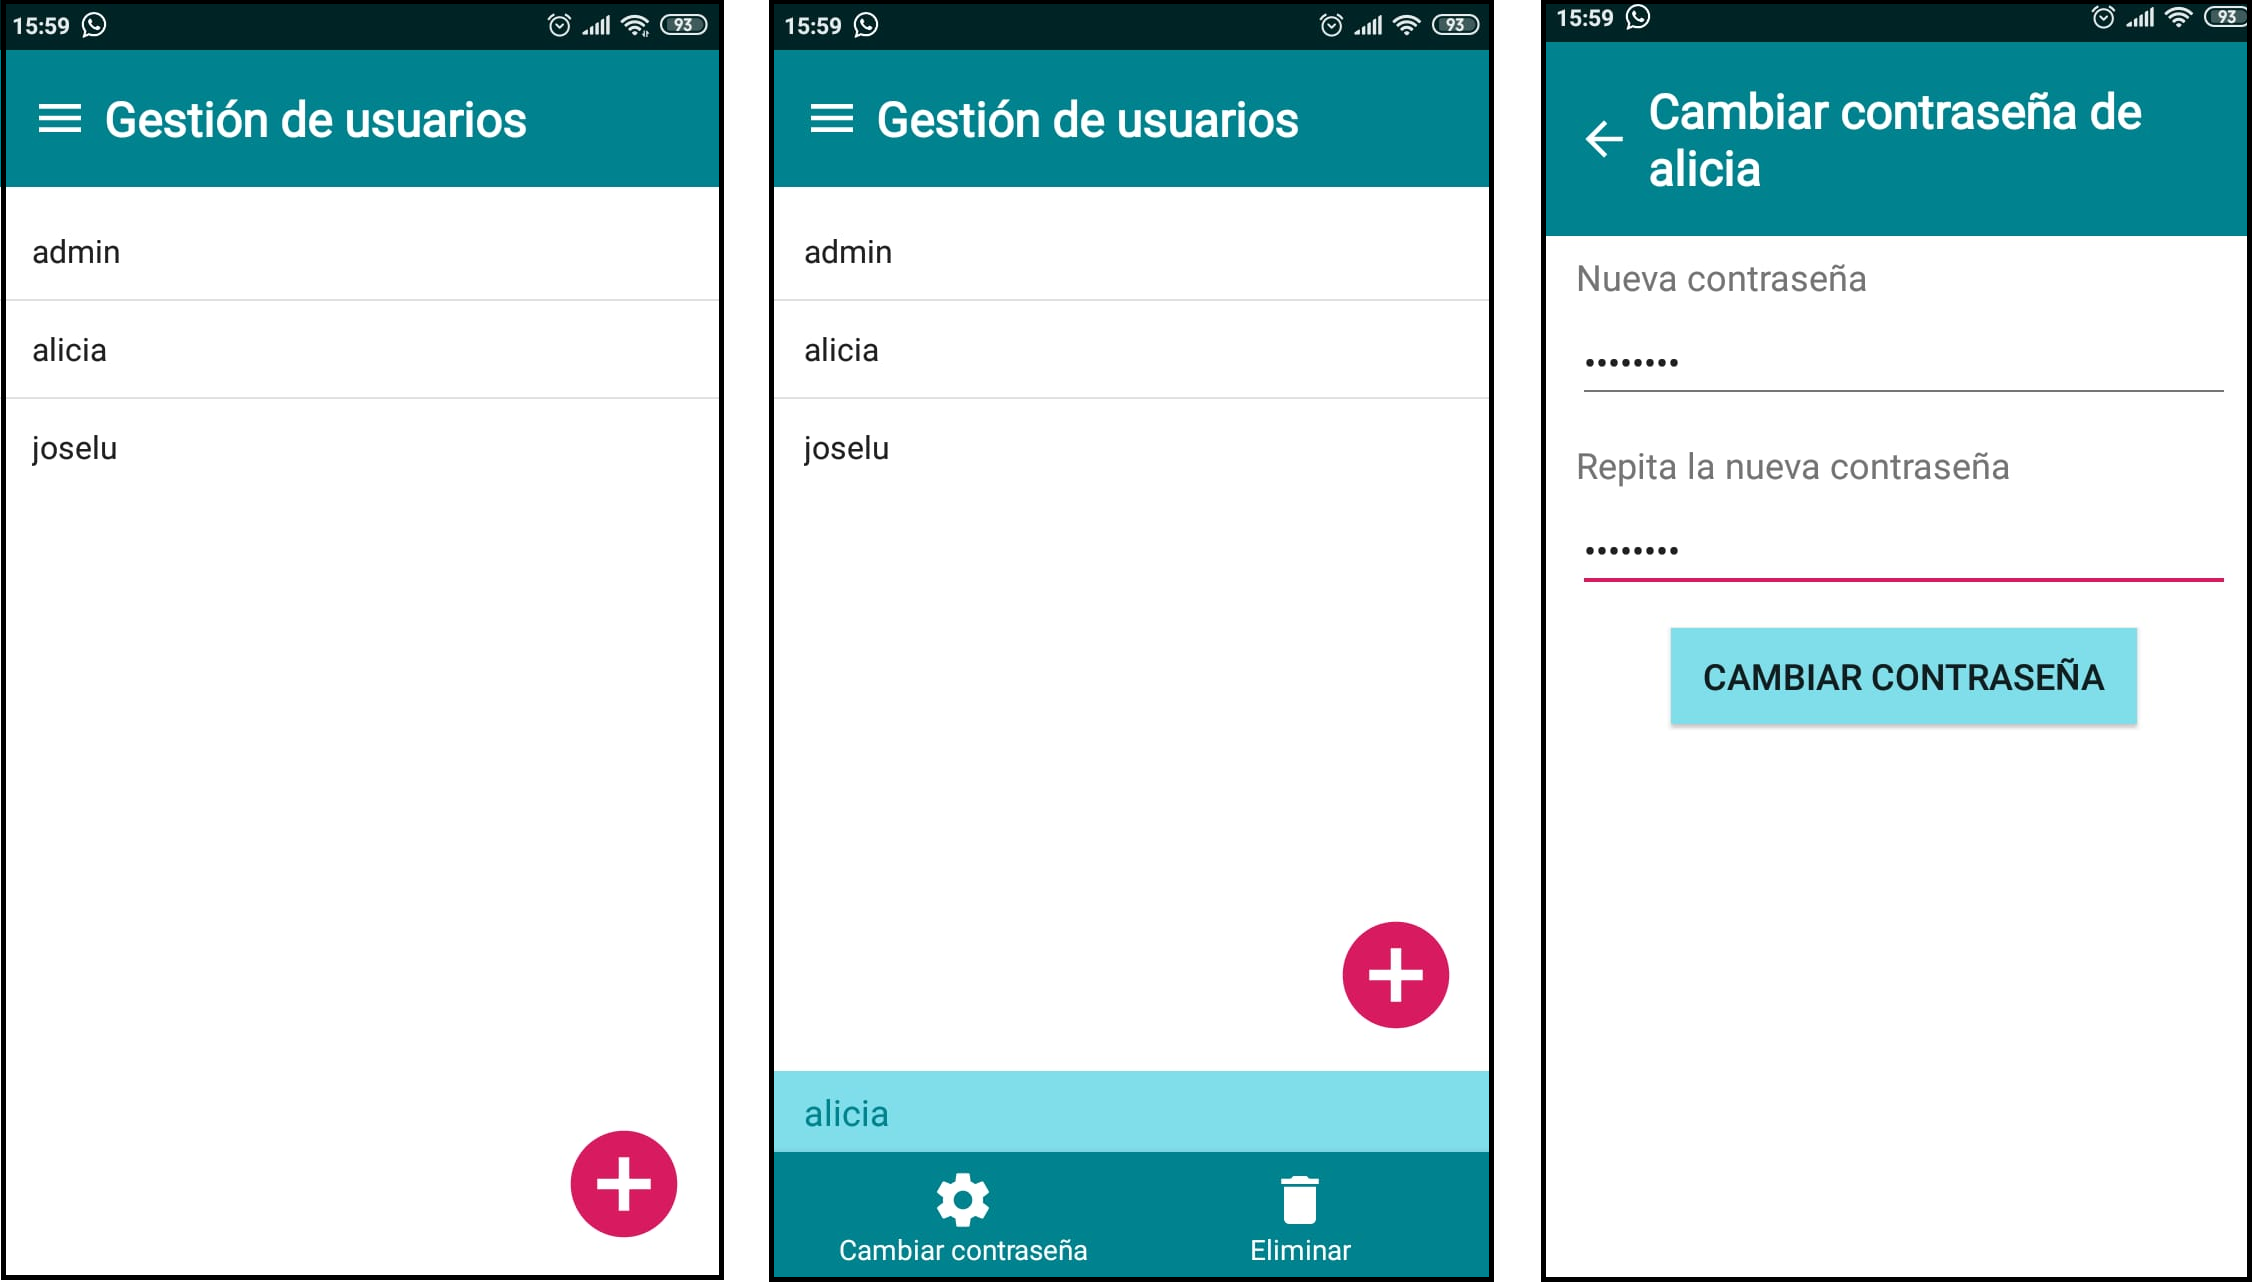
\includegraphics[width=1\textwidth]{../img/gestiondeusuarios.png}
	\caption{Gestión de usuarios, cambiar contraseña.}
	\label{fig:gestiondeusuarios}
\end{figure}

\begin{figure}[H]
	\centering
	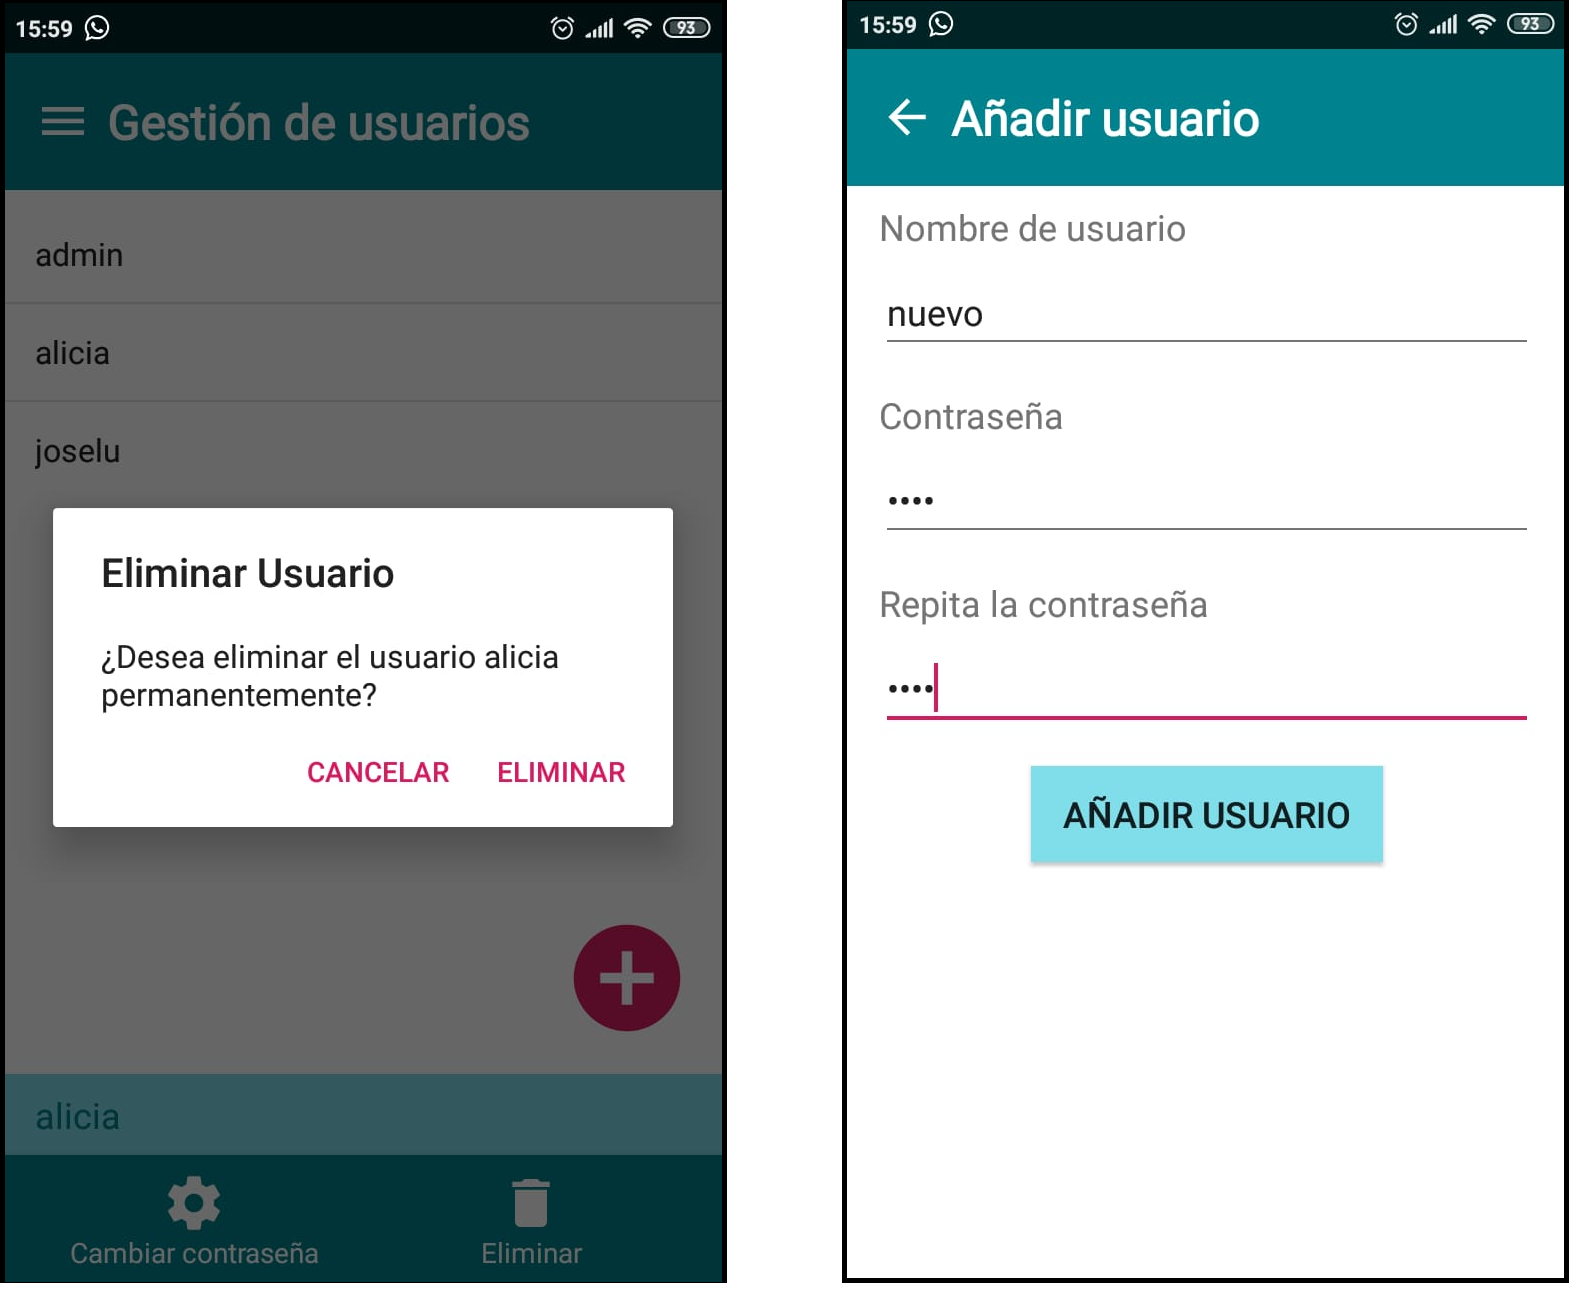
\includegraphics[width=0.7\textwidth]{../img/eliminaranadir.png}
	\caption{Gestión de usuarios, eliminar y añadir usuarios.}
	\label{fig:eliminaranadir}
\end{figure}
